% Options for packages loaded elsewhere
\PassOptionsToPackage{unicode}{hyperref}
\PassOptionsToPackage{hyphens}{url}
\PassOptionsToPackage{dvipsnames,svgnames,x11names}{xcolor}
%
\documentclass[
  11pt,
]{article}

\usepackage{amsmath,amssymb}
\usepackage{setspace}
\usepackage{iftex}
\ifPDFTeX
  \usepackage[T1]{fontenc}
  \usepackage[utf8]{inputenc}
  \usepackage{textcomp} % provide euro and other symbols
\else % if luatex or xetex
  \usepackage{unicode-math}
  \defaultfontfeatures{Scale=MatchLowercase}
  \defaultfontfeatures[\rmfamily]{Ligatures=TeX,Scale=1}
\fi
\usepackage{lmodern}
\ifPDFTeX\else  
    % xetex/luatex font selection
\fi
% Use upquote if available, for straight quotes in verbatim environments
\IfFileExists{upquote.sty}{\usepackage{upquote}}{}
\IfFileExists{microtype.sty}{% use microtype if available
  \usepackage[]{microtype}
  \UseMicrotypeSet[protrusion]{basicmath} % disable protrusion for tt fonts
}{}
\makeatletter
\@ifundefined{KOMAClassName}{% if non-KOMA class
  \IfFileExists{parskip.sty}{%
    \usepackage{parskip}
  }{% else
    \setlength{\parindent}{0pt}
    \setlength{\parskip}{6pt plus 2pt minus 1pt}}
}{% if KOMA class
  \KOMAoptions{parskip=half}}
\makeatother
\usepackage{xcolor}
\usepackage[margin=1in]{geometry}
\setlength{\emergencystretch}{3em} % prevent overfull lines
\setcounter{secnumdepth}{5}
% Make \paragraph and \subparagraph free-standing
\makeatletter
\ifx\paragraph\undefined\else
  \let\oldparagraph\paragraph
  \renewcommand{\paragraph}{
    \@ifstar
      \xxxParagraphStar
      \xxxParagraphNoStar
  }
  \newcommand{\xxxParagraphStar}[1]{\oldparagraph*{#1}\mbox{}}
  \newcommand{\xxxParagraphNoStar}[1]{\oldparagraph{#1}\mbox{}}
\fi
\ifx\subparagraph\undefined\else
  \let\oldsubparagraph\subparagraph
  \renewcommand{\subparagraph}{
    \@ifstar
      \xxxSubParagraphStar
      \xxxSubParagraphNoStar
  }
  \newcommand{\xxxSubParagraphStar}[1]{\oldsubparagraph*{#1}\mbox{}}
  \newcommand{\xxxSubParagraphNoStar}[1]{\oldsubparagraph{#1}\mbox{}}
\fi
\makeatother


\providecommand{\tightlist}{%
  \setlength{\itemsep}{0pt}\setlength{\parskip}{0pt}}\usepackage{longtable,booktabs,array}
\usepackage{calc} % for calculating minipage widths
% Correct order of tables after \paragraph or \subparagraph
\usepackage{etoolbox}
\makeatletter
\patchcmd\longtable{\par}{\if@noskipsec\mbox{}\fi\par}{}{}
\makeatother
% Allow footnotes in longtable head/foot
\IfFileExists{footnotehyper.sty}{\usepackage{footnotehyper}}{\usepackage{footnote}}
\makesavenoteenv{longtable}
\usepackage{graphicx}
\makeatletter
\def\maxwidth{\ifdim\Gin@nat@width>\linewidth\linewidth\else\Gin@nat@width\fi}
\def\maxheight{\ifdim\Gin@nat@height>\textheight\textheight\else\Gin@nat@height\fi}
\makeatother
% Scale images if necessary, so that they will not overflow the page
% margins by default, and it is still possible to overwrite the defaults
% using explicit options in \includegraphics[width, height, ...]{}
\setkeys{Gin}{width=\maxwidth,height=\maxheight,keepaspectratio}
% Set default figure placement to htbp
\makeatletter
\def\fps@figure{htbp}
\makeatother

\usepackage{hyperref}
\hypersetup{
  colorlinks=true,
  linkcolor=blue,
  urlcolor=blue,
  breaklinks=true,
  pdfborder={0 0 0}
}
\makeatletter
\@ifpackageloaded{caption}{}{\usepackage{caption}}
\AtBeginDocument{%
\ifdefined\contentsname
  \renewcommand*\contentsname{Table of contents}
\else
  \newcommand\contentsname{Table of contents}
\fi
\ifdefined\listfigurename
  \renewcommand*\listfigurename{List of Figures}
\else
  \newcommand\listfigurename{List of Figures}
\fi
\ifdefined\listtablename
  \renewcommand*\listtablename{List of Tables}
\else
  \newcommand\listtablename{List of Tables}
\fi
\ifdefined\figurename
  \renewcommand*\figurename{Figure}
\else
  \newcommand\figurename{Figure}
\fi
\ifdefined\tablename
  \renewcommand*\tablename{Table}
\else
  \newcommand\tablename{Table}
\fi
}
\@ifpackageloaded{float}{}{\usepackage{float}}
\floatstyle{ruled}
\@ifundefined{c@chapter}{\newfloat{codelisting}{h}{lop}}{\newfloat{codelisting}{h}{lop}[chapter]}
\floatname{codelisting}{Listing}
\newcommand*\listoflistings{\listof{codelisting}{List of Listings}}
\makeatother
\makeatletter
\makeatother
\makeatletter
\@ifpackageloaded{caption}{}{\usepackage{caption}}
\@ifpackageloaded{subcaption}{}{\usepackage{subcaption}}
\makeatother
\ifLuaTeX
  \usepackage{selnolig}  % disable illegal ligatures
\fi
\usepackage[]{biblatex}
\addbibresource{references.bib}
\usepackage{bookmark}

\IfFileExists{xurl.sty}{\usepackage{xurl}}{} % add URL line breaks if available
\urlstyle{same} % disable monospaced font for URLs
\hypersetup{
  pdftitle={William's Update},
  pdfauthor={William Clinton Co},
  colorlinks=true,
  linkcolor={blue},
  filecolor={Maroon},
  citecolor={blue},
  urlcolor={blue},
  pdfcreator={LaTeX via pandoc}}

\title{William's Update}
\usepackage{etoolbox}
\makeatletter
\providecommand{\subtitle}[1]{% add subtitle to \maketitle
  \apptocmd{\@title}{\par {\large #1 \par}}{}{}
}
\makeatother
\subtitle{Remittances}
\author{William Clinton Co}
\date{August 28, 2025}

\begin{document}
\maketitle
\begin{abstract}
This document is a follow-up to the meeting on August 21st and addresses
topics discussed during that meeting.
\end{abstract}

\renewcommand*\contentsname{Table of contents}
{
\hypersetup{linkcolor=}
\setcounter{tocdepth}{10}
\tableofcontents
}
\setstretch{1}
\section{Introduction}\label{introduction}

\section{Bitcoin Cross-Border Flows}\label{bitcoin-cross-border-flows}

\subsection{IMF}\label{imf}

Below is a comparison of the data challenges for remittances and Bitcoin
flows:

\begin{longtable}[]{@{}
  >{\raggedright\arraybackslash}p{(\columnwidth - 6\tabcolsep) * \real{0.0979}}
  >{\raggedright\arraybackslash}p{(\columnwidth - 6\tabcolsep) * \real{0.1538}}
  >{\raggedright\arraybackslash}p{(\columnwidth - 6\tabcolsep) * \real{0.3287}}
  >{\raggedright\arraybackslash}p{(\columnwidth - 6\tabcolsep) * \real{0.4196}}@{}}
\toprule\noalign{}
\begin{minipage}[b]{\linewidth}\raggedright
Channel
\end{minipage} & \begin{minipage}[b]{\linewidth}\raggedright
Data Observed
\end{minipage} & \begin{minipage}[b]{\linewidth}\raggedright
Data Missing/Challenge
\end{minipage} & \begin{minipage}[b]{\linewidth}\raggedright
Notes
\end{minipage} \\
\midrule\noalign{}
\endhead
\bottomrule\noalign{}
\endlastfoot
Remittances & Macro flows, location & Cannot obtain corridor-level
bilateral data; requires population inference & Can observe location,
but not detailed bilateral corridors \\
Bitcoin & Micro-level data & Cannot discern location; requires website
traffic inference & Public datasets available with sufficient
processing \\
\end{longtable}

For detailed information, see section 2 of\\
\href{https://drive.google.com/file/d/1JlapQvyER-SgX0z91l8NzTDcXR9Z5Oo5/view?usp=sharing}{A
Primer on Bitcoin Cross-Border Flows: Measurement and Drivers} This
document explains in detail how the process works. Bitcoin datasets are
publicly available with enough processing.

Below is one of the key images from the paper:

\begin{figure}[H]

{\centering 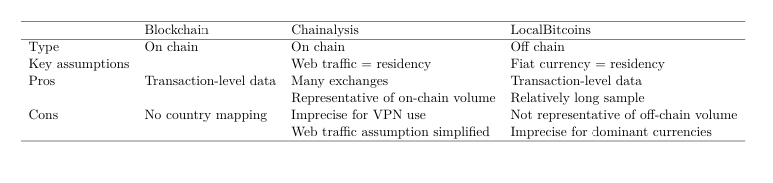
\includegraphics{images/Screenshot 2025-08-28 053010.png}

}

\caption{Key image from the paper}

\end{figure}%

\subsection{BIS}\label{bis}

\begin{itemize}
\tightlist
\item
  \href{https://www.bis.org/publ/work1265.pdf}{BIS Working Paper
  No.~1265}\\
\item
  \href{https://www.coinglass.com/news/471951?utm_source=chatgpt.com}{Coinglass
  News: Bitcoin Flows}
\end{itemize}

Key images from the BIS and Coinglass sources:

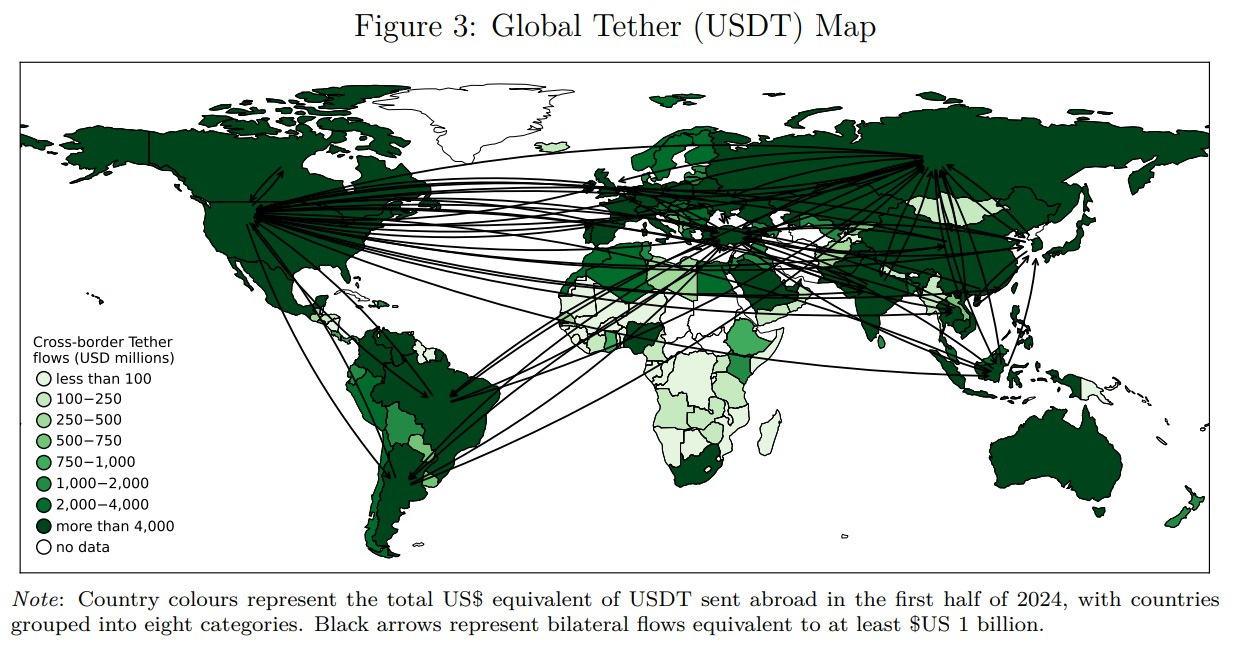
\includegraphics{C:/Users/clint/Desktop/RER/images/0196c41c-3a2a-7979-aab1-bab474641aa7.jpg}
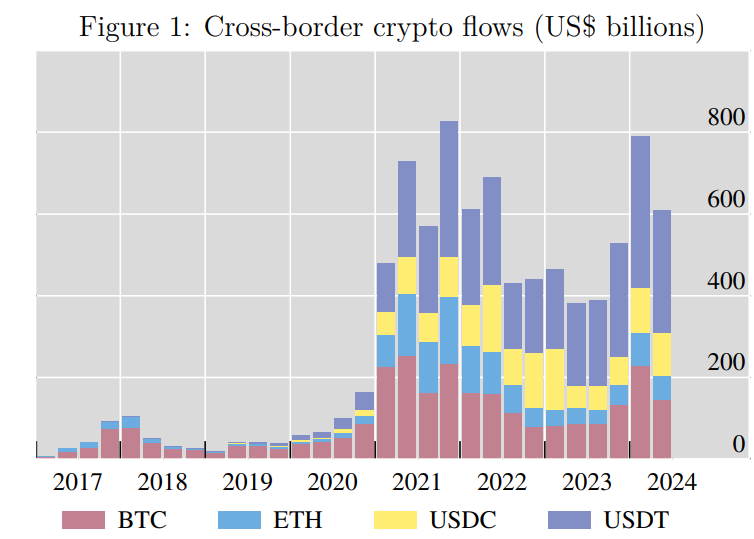
\includegraphics{C:/Users/clint/Desktop/RER/images/0196c41c-3696-7ce1-8a25-41b84deae178.png}

\section{Shocks}\label{shocks}

\begin{itemize}
\tightlist
\item
  \href{https://academic.oup.com/wber/article/21/2/219/1916657?login=true\#111402059}{Rainfall
  shocks}
\item
  \href{https://www.nber.org/system/files/working_papers/w12325/w12325.pdf}{Asian
  financial crisis shocks to exchange rates}
\end{itemize}

Potential shocks include:

\begin{itemize}
\tightlist
\item
  Crackdowns on illegal immigrants, which would reduce remittances.
\item
  Another interesting case is the Mexican Consular ID Card, issued in
  2002, which helped bolster remittances.
\end{itemize}

\begin{quote}
The Mexican government issues its nationals in the United States
official identity cards (matriculas consulares) that many financial
institutions accept as proof of identity for the purpose of opening a
bank account. If matriculas consulares lead to increases in migrant
savings rates and remittances sent home\ldots{}
\end{quote}

\section{Another Potential Remittance
Dataset}\label{another-potential-remittance-dataset}

\href{https://www.imf.org/en/Publications/WP/Issues/2021/07/16/Defying-the-Odds-Remittances-During-the-COVID-19-Pandemic-461321}{Defying
the Odds: Remittances During the COVID-19 Pandemic (IMF Working Paper)}

Attempts were made to contact the authors for further clarification
regarding their data construction process; only Saad Quayyum's contact
is publicly available. While the authors indicate that their dataset was
compiled from ``statistical institutes,'' the methodology for dataset
construction is not thoroughly detailed in the paper.

According to their paper:

\begin{quote}
To overcome these challenges, we compiled a new and unique dataset of
monthly remittance flows for a sample of 52 countries, of which 6 are
high-income countries, 35 are middle-income countries, and 11 are
low-income countries (see Annex 1 for the sample composition and data
sources). The time dimension of the data collected spans from January
2018 to December 2020. In addition, we gather monthly bilateral
remittance flows (corridor data) for 16 countries in the sample,
totaling 410 corridors. The data are extracted from detailed balance of
payments and statistical notes published by national central banks and
statistical institutes.
\end{quote}

\section{Appendix}\label{appendix}

\subsection{Shocks}\label{shocks-1}

\begin{itemize}
\tightlist
\item
  \href{https://www.investopedia.com/terms/m/mt-gox.asp}{What Was Mt.
  Gox? Definition, History, Collapse, and Future (Investopedia)}
\item
  \href{https://www.wsj.com/world/americas/el-salvador-made-bitcoin-an-official-currency-now-its-backtracking-for-imf-loan-874c6623}{El
  Salvador made Bitcoin an official currency, now it's backtracking for
  IMF loan (WSJ)}
\item
  \href{https://thetokener.com/learn/el-salvadors-bitcoin-story/}{El
  Salvador's Bitcoin Story (The Tokener)}
\item
  \href{https://crypto.news/china-crypto-bans-a-complete-history/}{China
  Crypto Bans: A Complete History (Crypto.news)}
\end{itemize}

\subsection{Bitcoin Datasets}\label{bitcoin-datasets}

There exist numerous Bitcoin datasets, each employing distinct
methodologies for data collection and analysis. Below are a few notable
examples:

\begin{itemize}
\tightlist
\item
  \href{https://arxiv.org/abs/2204.05746?utm_source}{BABD: A Bitcoin
  Address Behavior Dataset for Pattern Analysis}
\item
  \href{https://www.nature.com/articles/s41597-025-04595-8}{A Temporal
  Graph Dataset of Bitcoin Entity-Entity Transactions}
\end{itemize}

\subsection{Alternative Remittance
Channel}\label{alternative-remittance-channel}

\begin{itemize}
\tightlist
\item
  \href{https://www.econstor.eu/bitstream/10419/204586/1/1678825786.pdf}{Alternative
  Remittance Systems and Terrorism Financing: Issues in Risk Management}
\end{itemize}


\printbibliography


\end{document}
